%
% This work is based on the samplepaper.tex template.
% Version 2.20 of 2017/10/04
%

\documentclass[runningheads]{llncs}
\renewcommand{\thesection}{\Roman{section}}

\usepackage[dvipsnames]{xcolor}
\usepackage{graphicx}
\usepackage{color}
\usepackage[colorinlistoftodos]{todonotes}
\usepackage[normalem]{ulem}
\usepackage[acronym]{glossaries}
\usepackage{xargs}

% @Cristian You can you use this kind of stuff to define your own TODO colors,
% and then it's easy to call from text. Like this:
% \todoglg{<some text>}

\newcommandx{\todoglg}[2][1=]{\todo[
	linecolor=ForestGreen,
	backgroundcolor=ForestGreen!25,
	bordercolor=ForestGreen,
	#1]{#2}}

% If you use the hyperref package, please uncomment the following line
% to display URLs in blue roman font according to Springer's eBook style:
% \renewcommand\UrlFont{\color{blue}\rmfamily}

\begin{document}

\title{Contribution Title\thanks{Supported by organization x.}}
%
%\titlerunning{Abbreviated paper title}
% If the paper title is too long for the running head, you can set
% an abbreviated paper title here
%

\author{First Author\inst{1}\orcidID{0000-1111-2222-3333} \and
Second Author\inst{2,3}\orcidID{1111-2222-3333-4444} \and
Third Author\inst{3}\orcidID{2222--3333-4444-5555}}
%
\authorrunning{F. Author et al.}
% First names are abbreviated in the running head.
% If there are more than two authors, 'et al.' is used.
%
\institute{Princeton University, Princeton NJ 08544, USA \and
Springer Heidelberg, Tiergartenstr. 17, 69121 Heidelberg, Germany
\email{lncs@springer.com}\\
\url{http://www.springer.com/gp/computer-science/lncs} \and
ABC Institute, Rupert-Karls-University Heidelberg, Heidelberg, Germany\\
\email{\{abc,lncs\}@uni-heidelberg.de}}
%
\maketitle              % typeset the header of the contribution
%

\begin{abstract}

{\color{blue} In this paper, we present a framework to make available the car
information through an embedded wireless network. Working on the Open Source
Vehicle platform, we developed a program to read car data (such as speed,
battery level, etc), and we build a RPL network with a CoAP server to make these
data available to other modules of the car. We developed wireless receivers to
retrieve these information and display them in 3D printed devices..}.

\keywords{First keyword  \and Second keyword \and Another keyword.}
\end{abstract}
%

%

% List of acronyms.
% TODO Not sure where to put this.
\newacronym{osv}{OSV}{Open-Source Vehicle}
\newacronym{bms}{BMS}{Battery Management System}
\newacronym{ec}{EC}{Engine Controller}
\newacronym{soc}{SOC}{State of Charge}
\newacronym{wsn}{WSN}{Wireless Sensor Network}
\newacronym{coap}{CoAP}{Constrained Application Protocol}
\newacronym{rest}{REST}{Representational State Transfer}

\section{Introduction}

{\color{blue} Nowadays in the automotive industry, Controller Area Network bus (
CAN bus) technologies play a key role in coordinating the systems and subsystems
of every type of vehicle.
With an eye towards proposing an alternative to this technology, we develop, as
a proof of concept, an embedded wireless network using IoT protocol to run the
dashboard of the OSVehicle. Furthermore, we replace the TSCH default scheduling
for a custom one that better suits this particular network. }


%\section{Related Work}

\section{Architecture and Protocols}
\subsection{The Open-Source Vehicle electric car platform}

% FIXME @ALL This is probably because of the template, but the "subsubsection"
% does % not appear very clearly…

\subsubsection{Platform}

The main focus of our work is the \gls{osv} powertrain, which is 
{\color{blue}made of}
every system involved in generating power and transforming it into mechanical
forces. They are the Lithium-Ion battery, the \gls{bms}, the \gls{ec} 
{\color{blue}also}
often called Inverter, and the electric 3-phase AC engine. \\

The role of the \gls{bms} is to guarantee the safe and reliable battery
operation. It handles the measurement of its status, such as cell voltage,
current, and temperature. It {\color{blue}also} takes care of calculating the 
battery's
\gls{soc}, {\color{blue}and finally it can allow} the Charger and \gls{ec} to 
function.
This way, it can ensure the battery cells remain in their {\color{blue}safety 
window} (i.e.
their allowed voltage and temperature range).

%It determines charge/discharge limits at a given time; enables and disables
%charging; enables and disables the EC; and performs the cells balancing. \\

The \gls{ec}'s purpose is to generate 3-phase AC current for the engine, and
pilot its input voltage and torque
\todoglg{@GLG: Check if this actually voltage or current}
\todo{\color{blue} I think It uses  voltage/frequency feedback to control the 
sine-wave(engine speed)} \todo{\color{blue}I believe that torque is handled by 
transmission, and this is not part of the EC for what I understood. }
using a closed control loop.

%The \gls{ec} monitors and drives the
%motor.
%The EC consists of an AC drive controller that digitally process the vehicle's
%information and generates the switching signals necessary for the associated
%power electronic converter to do the corresponding DC/AC conversion.

Both of these components hold important data on the vehicle, and are capable of
exposing them to other devices.

%This devices are the core of the car's powertrain and the focus of this
%demonstration.


\begin{figure}[!h]
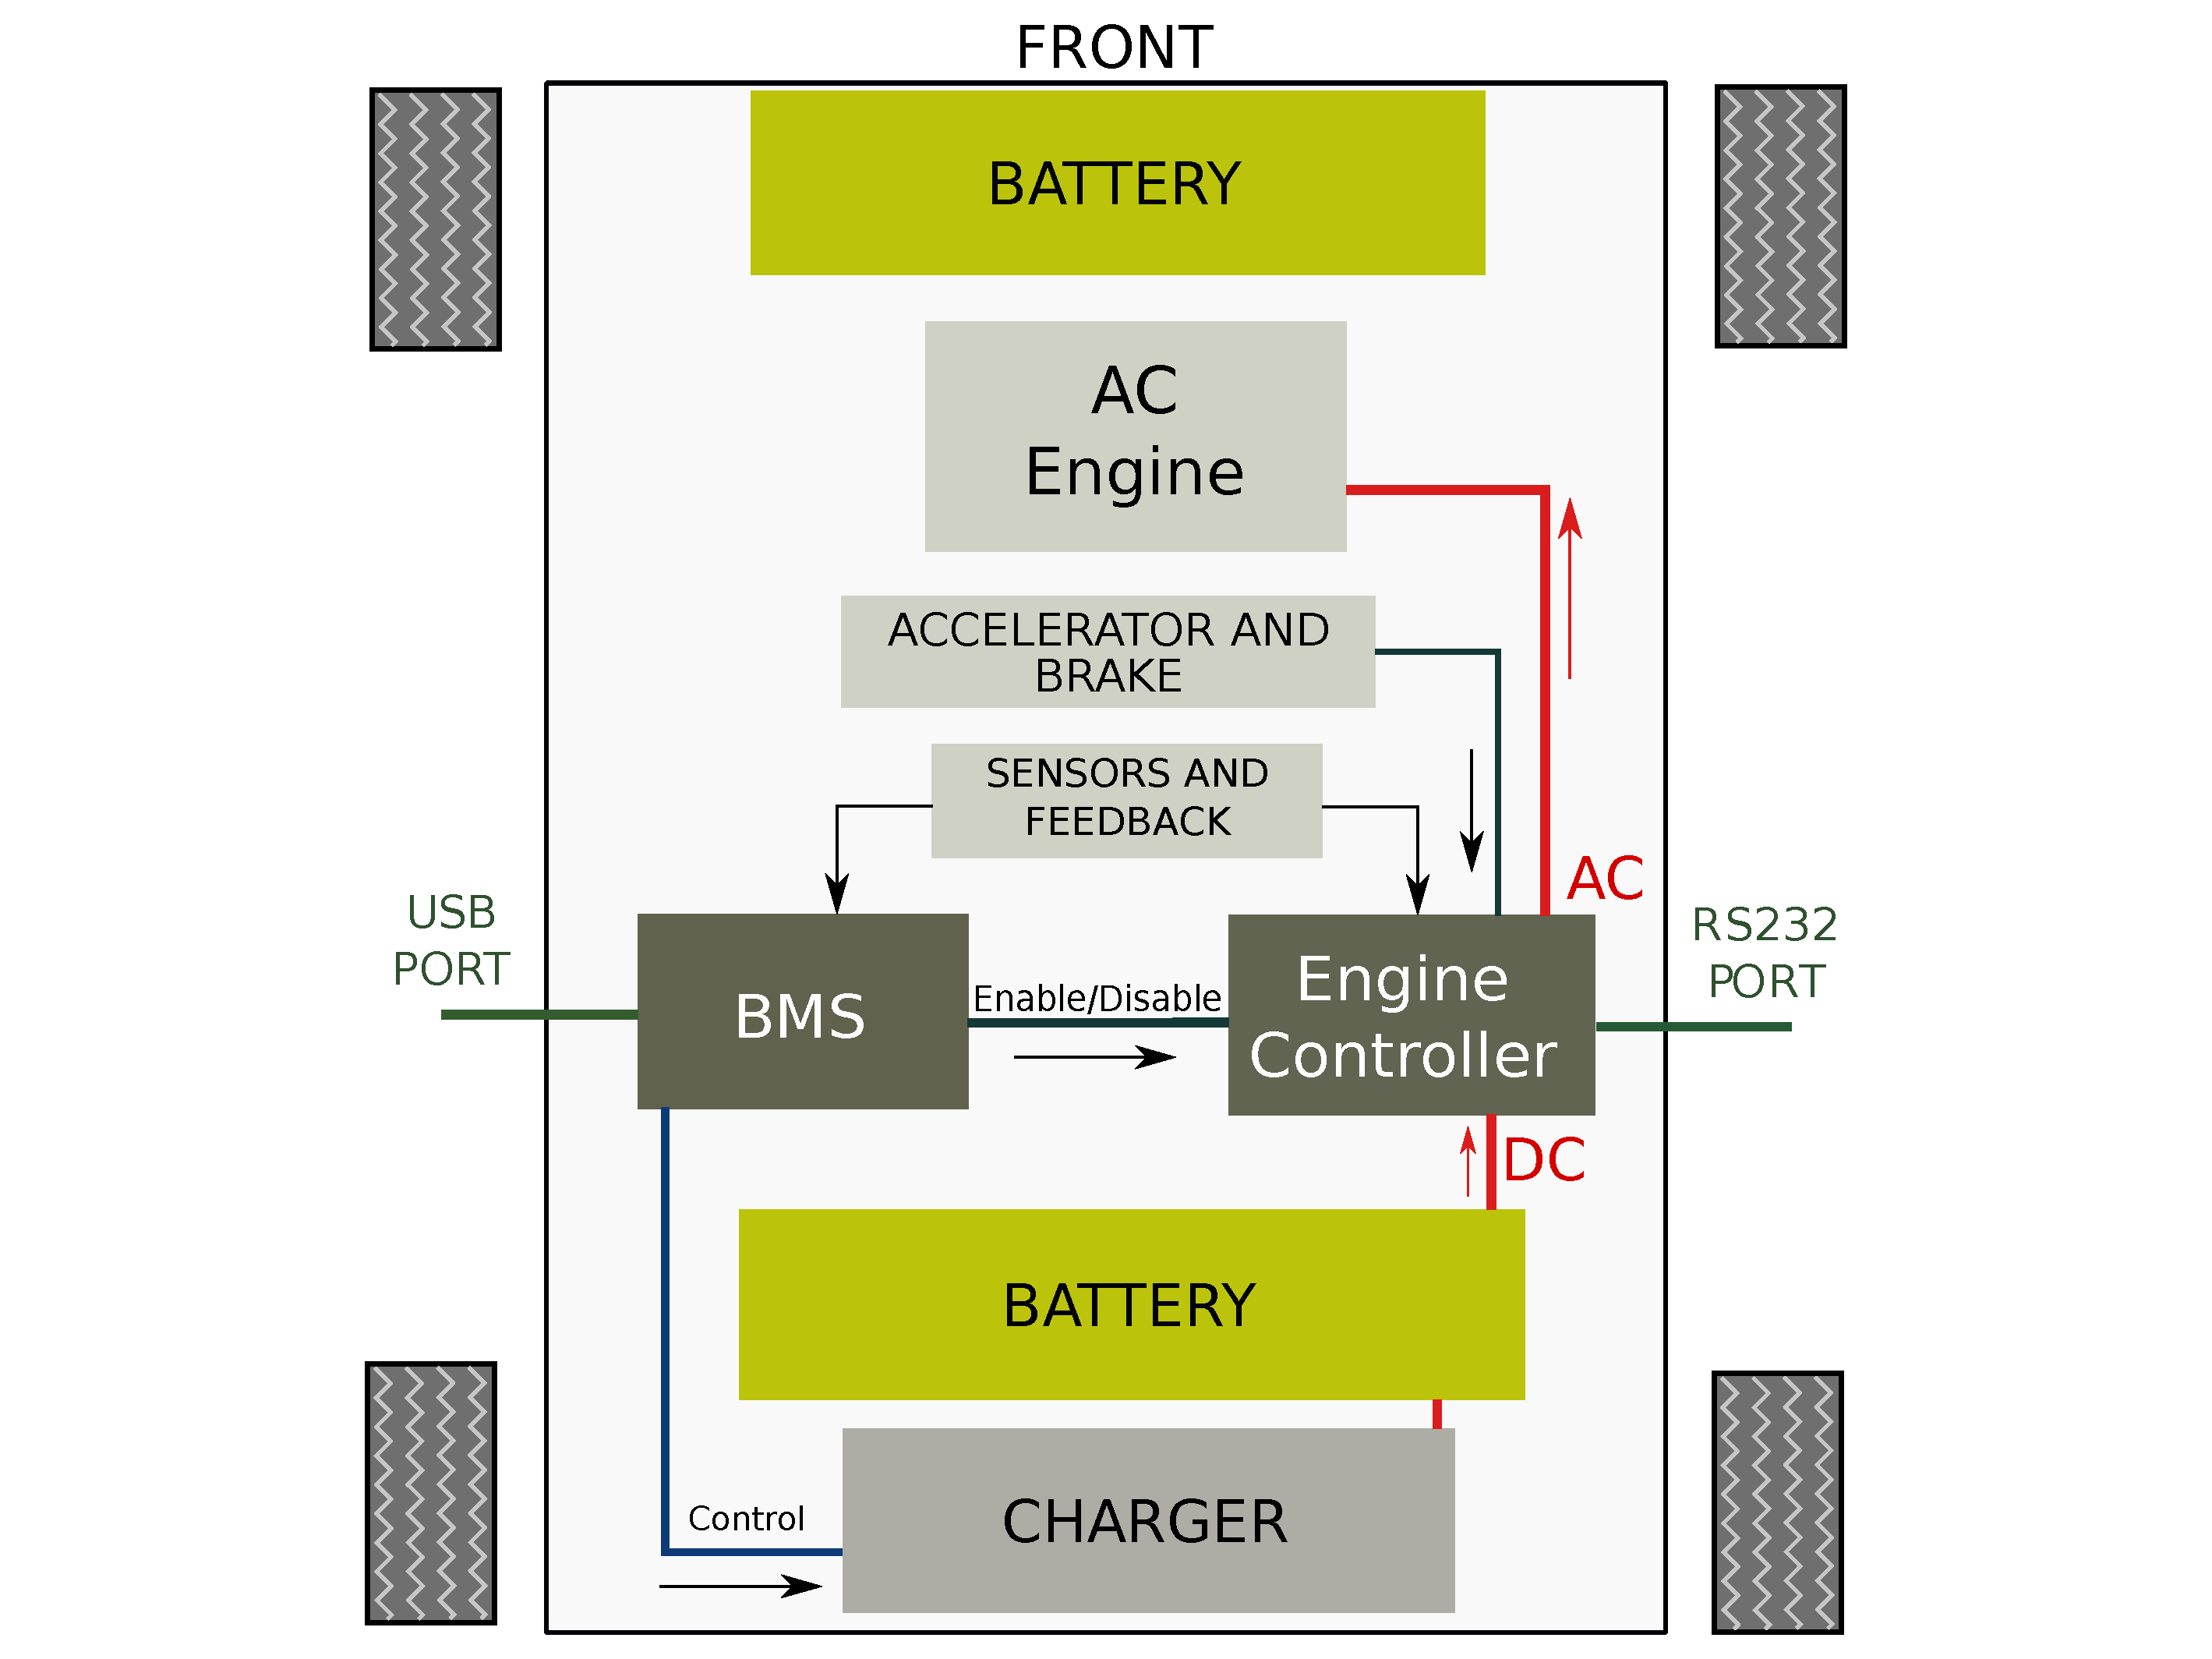
\includegraphics[width=\textwidth] {OSV.pdf}




\caption{The \gls{osv} platform: communication between the main systems}
\label{fig1}
\end{figure}

\subsubsection{Available Data}
%this is not here   Level of details dont't match (probable introduction)
%HOW DO I GET THE INFO, PORts, format and protocols.
%BMS CONECT AND EC CONNECT
	
Several data \todo {\color{blue} I think in english can't say just "several 
data"(i.e several data collections, several data points)}  can be retrieved 
from the OSV, most of them \todo{if not all?} 
from the \gls{bms} and \gls{ec}. Some of these data are usually exposed to the 
driver in real time (like the speed of the car, or the battery level of 
charge), while some others are usually for maintenance.
\todo{NM:I am wondering if we should not say somewhere that actually the OSV is really basic, in the sense that it is a platform for development and e.g. it does not have any diplays, nor roof, etc. Maybe in the intro?}
Table \ref{tab:data} gives a more details on the data we selected.
% TODO use LaTex references, not plain text to refer to tables / figures
Even though this information is contained in the devices \todo{NM: I don't understand what you mean here, the info is constrained?}, the original platform 
lacks displays to show it to users.

Both the \gls{bms} and \gls{ec} expose their available data through a custom 
ad-hoc protocol built on top of a UART connection. Each component is implementing 
its own protocol and data format.

The \gls{bms} protocol is a simple enable/disable data flow model: data stream 
starts when the reader device sends an enable command and stops when the 
disable command is sent. This has the disadvantage of requesting a whole data 
loop when just a few variables are needed.
On the other hand, the \gls{ec} implements a request/response communication 
protocol, meaning each variable is requested separately with a specific command.

Knowing this information, and the specifications of these protocols, it is
possible to build an in-vehicle network, to expose the powertrain's data to 
the rest of the vehicle devices.

\subsection{Wireless Networks State of the Art}

\todo {\color{blue} trying to introduce the protocols, but it might not be a
good title "State of the art" since we are just mentioning the ones we will use}
\todoglg{@Cristian Agreed. This is definitely not a state of the art. These are 
just the protocols we want to use. We need to search for another title here.}

% TODO This contains no meaningfull information. To be rephrased or removed.
\sout{As Internet of Things (IoT) and devices relying on it grow nowadays,
applications like Constrained Application Protocol ( CoAP ) are widely
spreading.}

One of the motivations of this work is to evaluate the benefits of exposing 
data through a \gls{rest} API for in-vehicle networking. And \gls{coap} is the 
go-to application protocol for such a framework in a \gls{wsn}. It provides a 
request/response model between two endpoints. It uses a subset of HTTP request 
methods such as GET, PUT, POST, DELETE. Furthermore, \gls{coap} also offers 
extensions such as OBSERVE which allows the client to subscribe to a server's 
resource and get notified when a it changes.

On lower layers in the network stack, UDP is used as the transport layer 
because it is mandated by the \gls{coap} standard.
6LoWPAN IPv6 is commonly used to build Low-power Lossy-Networks (LLNs).

IP routing is handled with RPL and enabled through the 6TiSCH mode of IEEE
802.15.4e. {\color{blue} This staet of the art network stack is the base for our
in-vehicle network architecture.}
	
%Check size, details and add Image Index (i.e) Image 1
\subsection{Proposed Architecture}
% HOW DO I MAKE IT AVAILABLE!??  (NOT TALK ABOUT OPENMOTE or HARDWARE.. contiki
% either )
Figure 2 illustrates the functional diagram of the proposed architecture.
In this scenario we distinguish two main blocks. The transmitter side, where
the information from the powertrain is retrieved, processed and then stored in
the COAP server; and the receiver side where the client requests the information
using GET or OBSERVE CoAP methods and forwards it to the displays handler.

% make the new Figure 3.



%  Check this


\begin{figure}[!h]
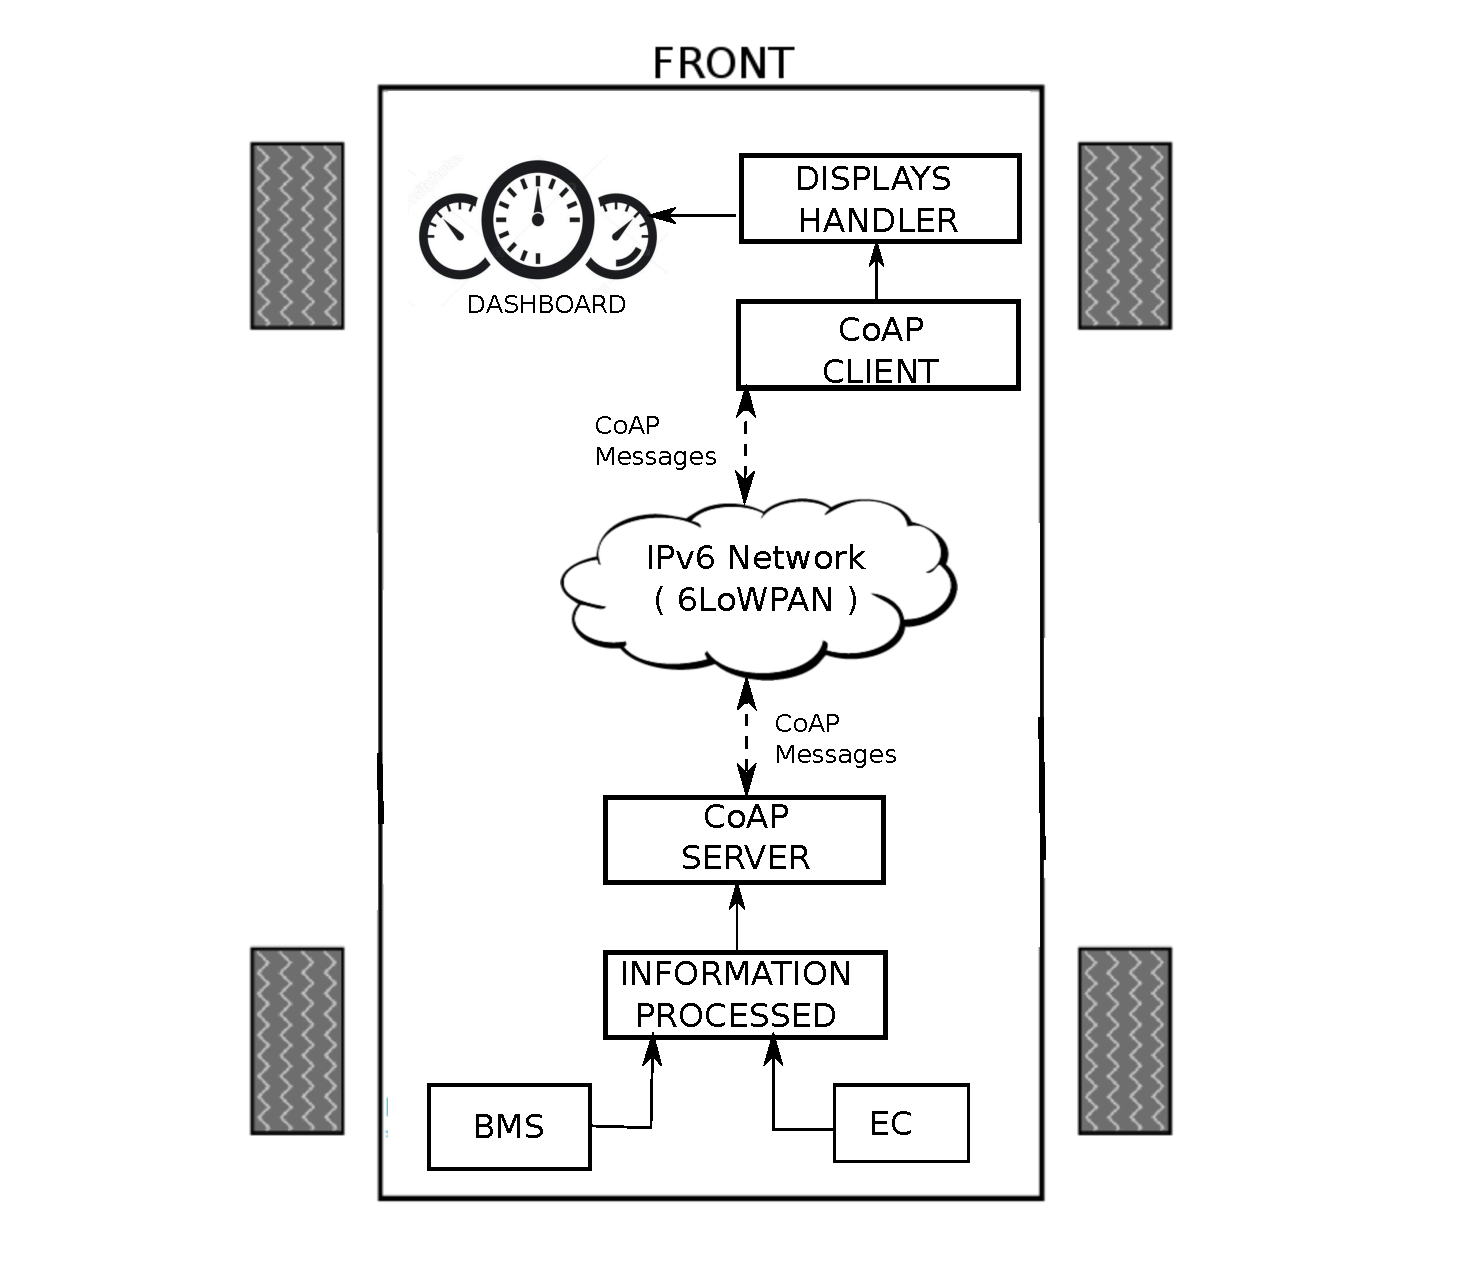
\includegraphics[width=\textwidth] {Information_Flow_Network.pdf}

\caption{Data flow from BMS and EC to DASHBOARD} \label{fig2}
\end{figure}


\section{Demonstration}
\subsection{Hardware}


As an implementation of the ideas presented so far, we developed the
full architecture shown in Fig 3, which exposes the hardware as well as the low
level protocols involved.

To interface the powertrain and the transmitter we used an Arduino DUE. It's
powerful micro-controller supports USB hosting to talk to the BMS as well as
UART ports to communicate the EC. It also offers a variety of other ports to
eventually perform other connections.

As shown in figure 3, the other Arduino acts as a displays handler. Since this
Arduino platforms are  widespread, it is easy to use them as hardware interfaces
and focus on the wireless communication devices.
	
Finally, to perform the wireless communication, two OpenMotes CC2538 were
selected to be the transmitting and receiving devices. This low power module
supports the protocol stack proposed above running  on Contiki OS. It also
provides the serial ports necessary to communicate with other modules.

Note that voltage shifters are needed to avoid voltage level mismatches when
interconnecting the chosen hardware.

\begin{figure}[!h]
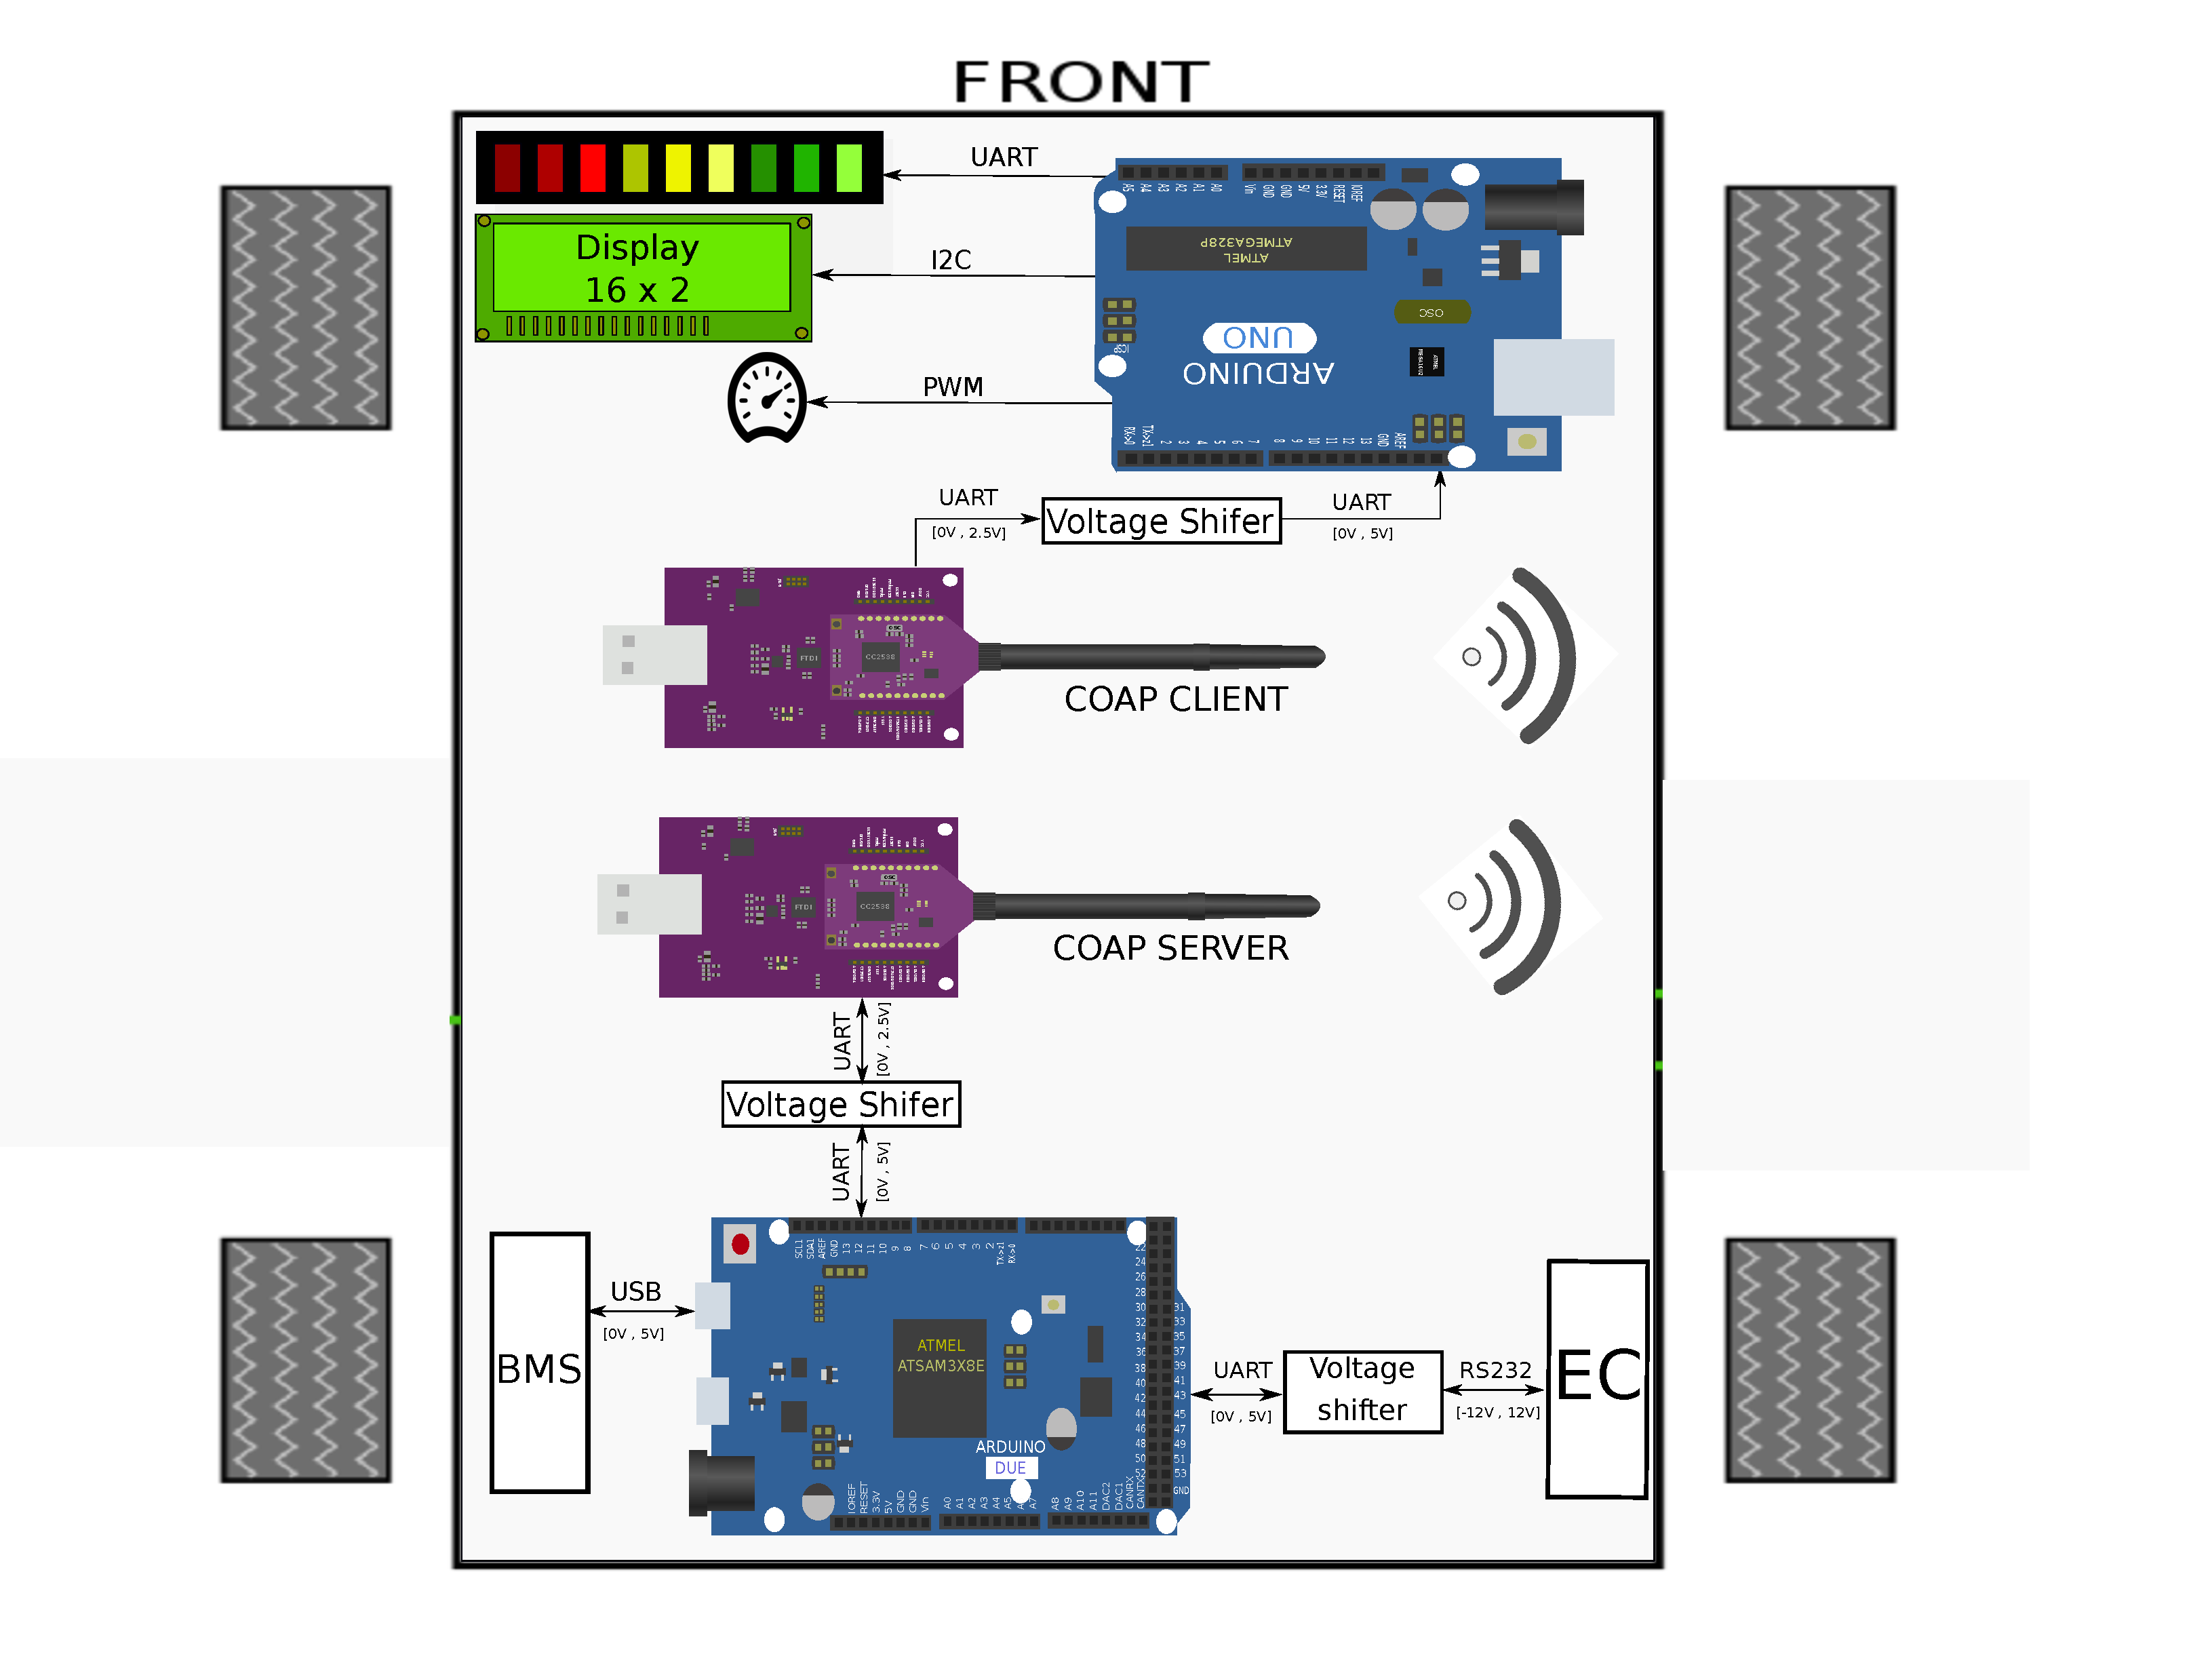
\includegraphics[width=\textwidth] {proposed_architecture_UNO.pdf}

\caption{Proposed architecture for this demonstration} \label{fig2}
\end{figure}


\subsection{Resource Management}
	
Since resources may have unpredictable behavior, this demonstration takes
advantage of the Observing Resource COAP protocol extension. This feature allows
us make smart decisions on when and how to update the server's information and
automatically notify client.
For this matter, we optimize the interface's program to make smart requests
by analyzing key relations between the resources. For example, if the car is not
moving , wait for a change in speed to update distance, or if the car is
charging, do not request speed or distance at all until charging condition turns
OFF.

As mentioned before, the data needs to be parsed to obtain the actual value of
the variable requested. For this purpose we implemented a program that extracts
this value and adds a key to it (``km",``km/h", etc.). This way the information
follows a uniform format and can be stored in the server and offered to the
network.
The client simply forwards this data to the display handler who according to
the type of resource will update the corresponding display in the dashboard.

\begin{table}
\caption{Hardware involved in the demonstration architecture}\label{tab1}
\begin{tabular}{|l|l|l|}
\hline
Device & Ports used  &  { Main Task } \\
\hline

Arduino DUE  &  { UART1/I2C/USB-host }  &  { Interface }  \\
Arduino UNO &  { UART1/UART2/PWM/I2C } &  { Display Handler }\\
Openmote cc2538 REV-A1 & { I2C } &  { Transmit }\\
Openmote cc2538 REV-A1 & { UART } &  { Receive } \\
LCD Display & { I2C } &  { Display Km,$^{\circ}C$, V}\\
Servo-motor & { PWM }  &  { Display Km/h }\\
Bar Led Display & { UART } &  { Display SoC}  \\
\hline
\end{tabular}
\end{table}

\begin{table}
\caption{Resources Management}\label{tab1}
\begin{tabular}{|l|l|l|l|}
\hline
Resource & Origin  & Request type & Server Update Strategy\\
\hline

Speed &  { E.C } & Subscription & Conditioned by Charging \\
SoC  & { B.M.S} & Subscription& Conditioned by Speed and Charging\\
Distance & { E.C } & Subscription & Conditioned by Speed\\
Charging & { B.M.S}  & Subscription & Conditioned by Speed\\
Temperature & { B.M.S}  & Subscription & Periodically \\
Cells Voltage & { B.M.S}  & Periodically & Periodically \\
\hline
\end{tabular}
\label{tab:data}
\end{table}

\paragraph{}
\paragraph{}
\paragraph{}

\section{Conclusion}
\paragraph{}
\paragraph{}




%/////////////////////////////////////////////////////////////////////////////////
%COPY FOR REFERENCE (EXAMPLE)



% ---- Bibliography ----
%
% BibTeX users should specify bibliography style 'splncs04'.
% References will then be sorted and formatted in the correct style.
%
% \bibliographystyle{splncs04}
% \bibliography{mybibliography}
%
\begin{thebibliography}{8}
\bibitem{ref_article1}
Author, F.: Article title. Journal \textbf{2}(5), 99--110 (2016)

\bibitem{ref_lncs1}
Author, F., Author, S.: Title of a proceedings paper. In: Editor,
F., Editor, S. (eds.) CONFERENCE 2016, LNCS, vol. 9999, pp. 1--13.
Springer, Heidelberg (2016). \doi{10.10007/1234567890}

\bibitem{ref_book1}
Author, F., Author, S., Author, T.: Book title. 2nd edn. Publisher,
Location (1999)

\bibitem{ref_proc1}
Author, A.-B.: Contribution title. In: 9th International Proceedings
on Proceedings, pp. 1--2. Publisher, Location (2010)

\bibitem{ref_url1}
LNCS Homepage, \url{http://www.springer.com/lncs}. Last accessed 4
Oct 2017
\end{thebibliography}
\end{document}

